\chapter{Lab 8: Memory} \label{day8}

\section{Memory module}

This module can store and output stored information. The data to be stored is received using the ``UART''-receiver module from the previous lab and then read out from the memory and displayed on the display of the \gls{fpga} board after pressing a button. 

The module can store 256 bytes. After 256 bytes the write address overflows and starts to overwrite information. The read address can be selected with switches and displayed after pressing a button.

\lstinputlisting[language=VHDL]{./L8/E1/src/project_8_1.vhd}

\lstinputlisting[language=VHDL]{./L8/E1/src/project_8_1_1.vhd}

\section{LIFO/stack}

The ``LIFO'' stack works as follows: The last stored information ist the first to be output. We use it here to display the received information from the computer keyboard on the display of the \gls{fpga} after pressing the button.

\lstinputlisting[language=VHDL]{./L8/E2/src/project_8_2.vhd}

\lstinputlisting[language=VHDL]{./L8/E2/src/project_8_2_1.vhd}

Additionally we test several borderline cases: 

\begin{itemize}
    \item reading from an empty stack
    \item writing to a full stack
    \item simultaneous reading and writing (starting with a full/empty stack)
\end{itemize}

\begin{figure}
    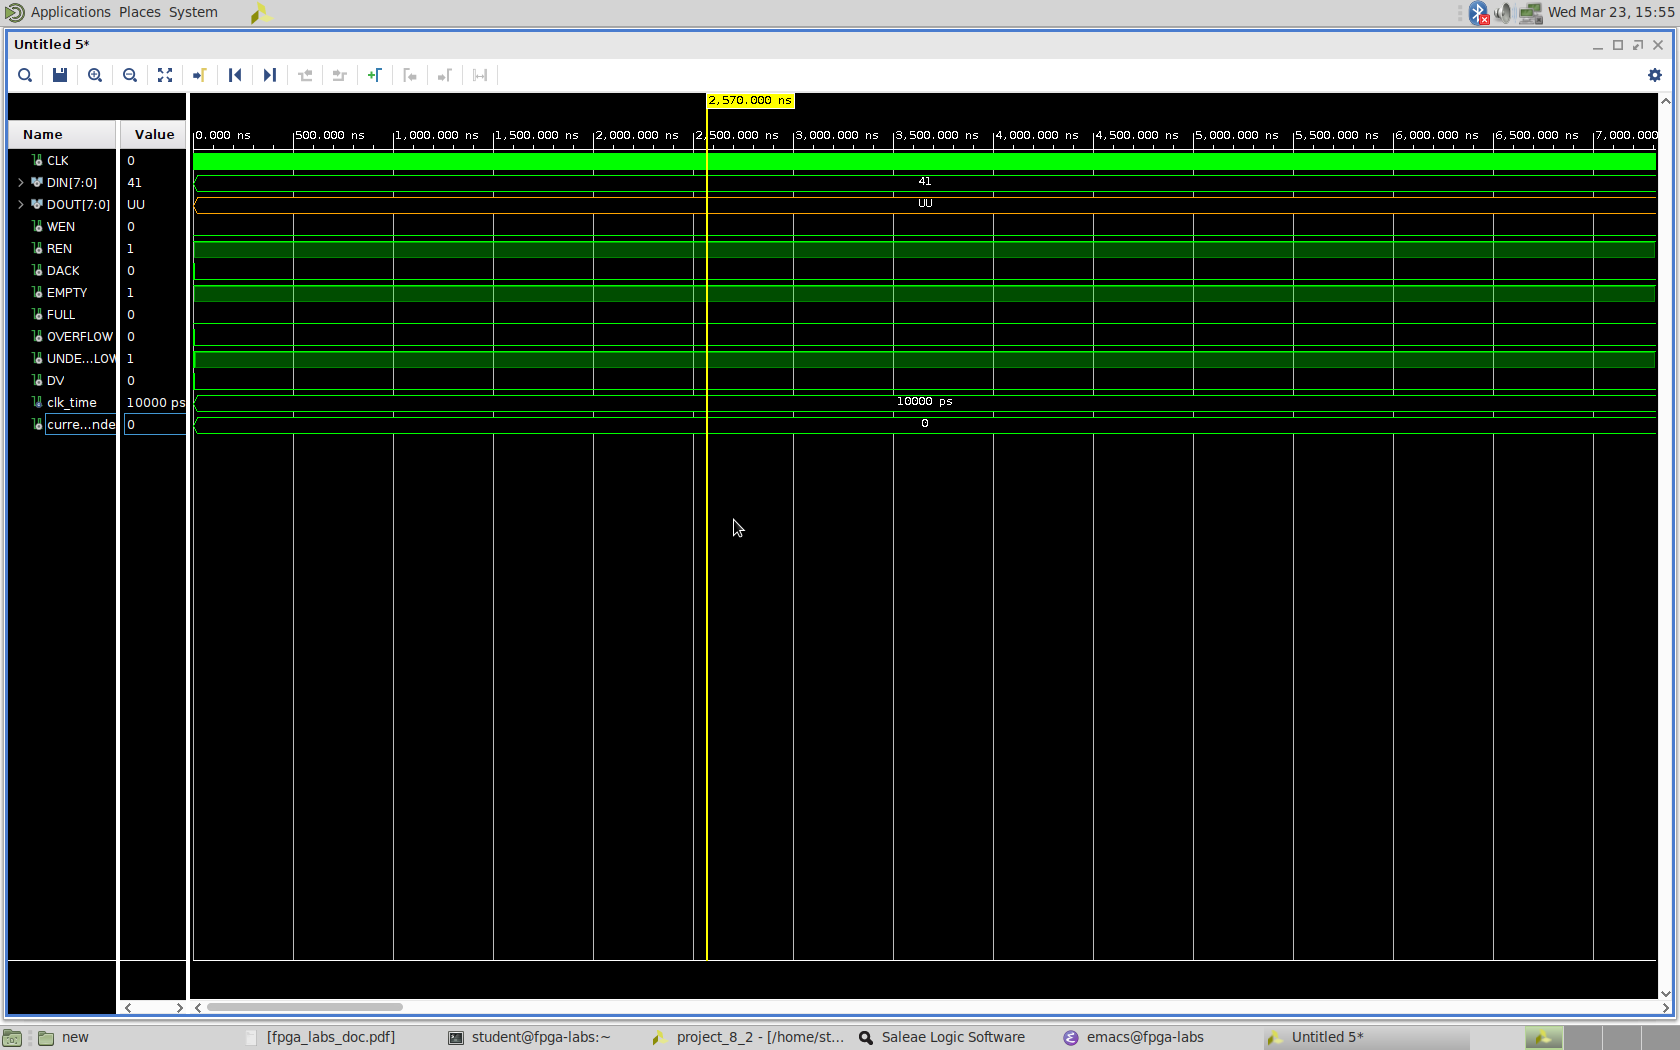
\includegraphics[width=\textwidth]{L8/E2/underflow.png}
    \caption{Reading from an empty stack. The stack underflows.}
    \label{pic: reading from an empty stack}
\end{figure}

\begin{figure}
    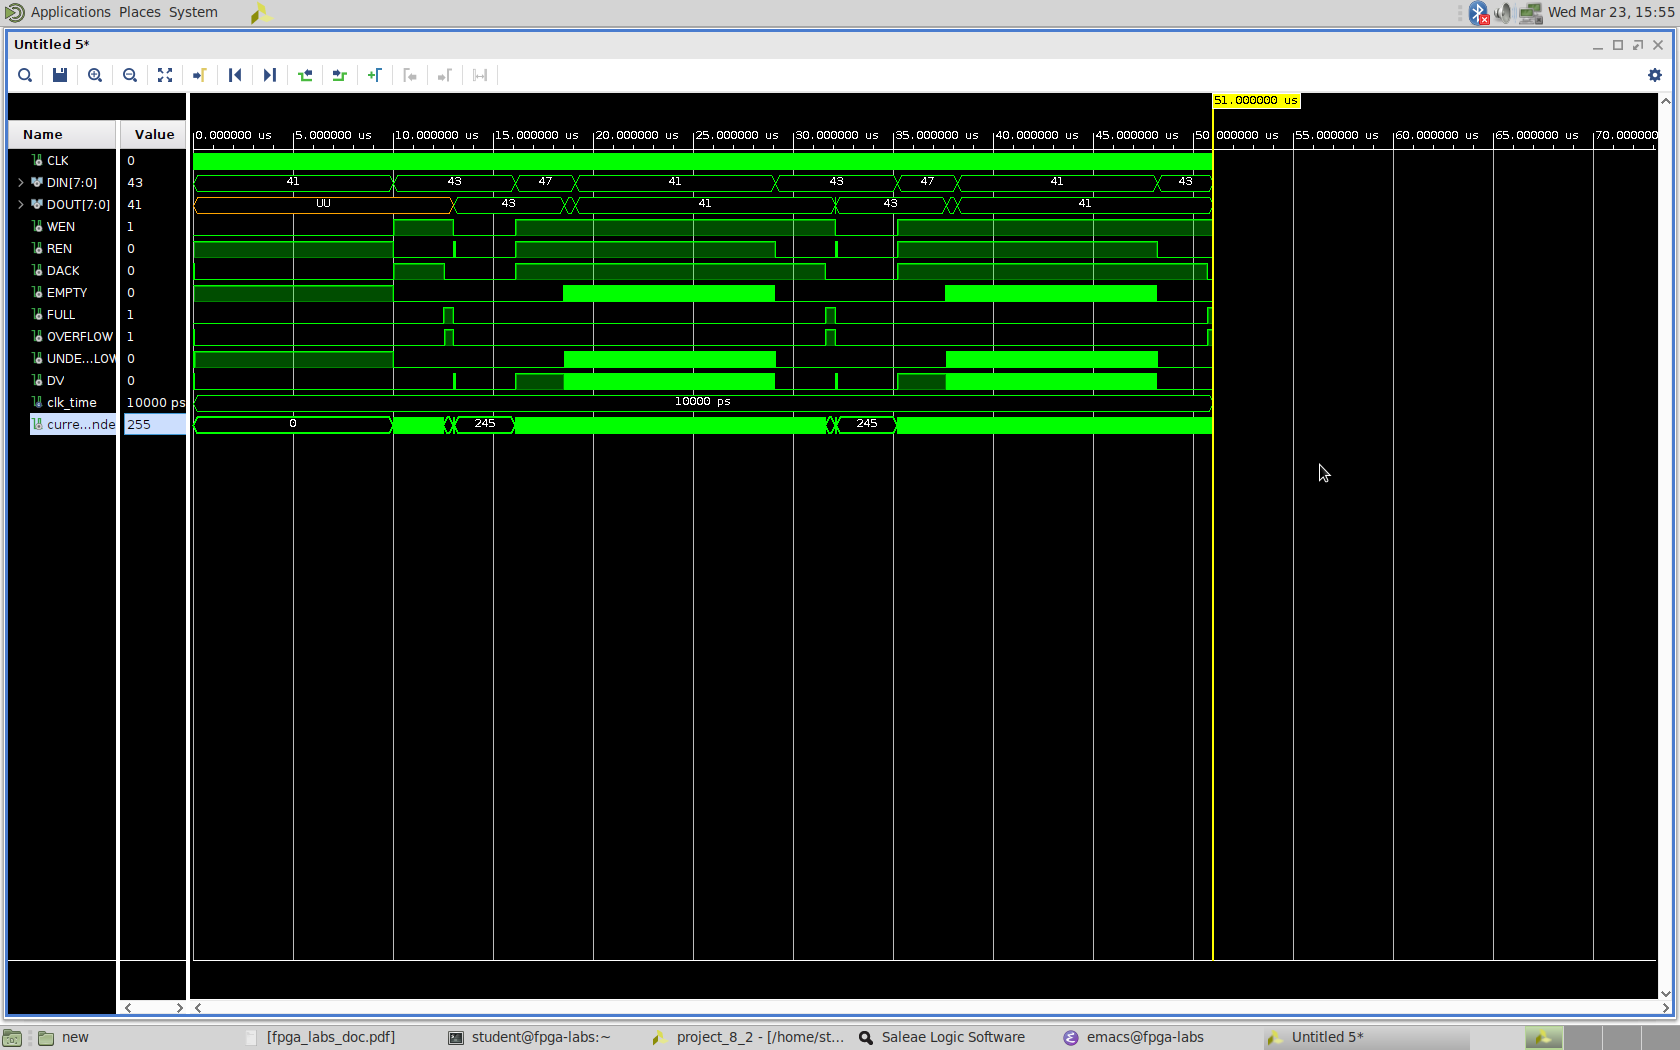
\includegraphics[width=\textwidth]{L8/E2/full.png}
    \caption{Writing to a full stack. The stack overflows and information is overwritten.}
    \label{pic: writing to a full stack}
\end{figure}

\begin{figure}
    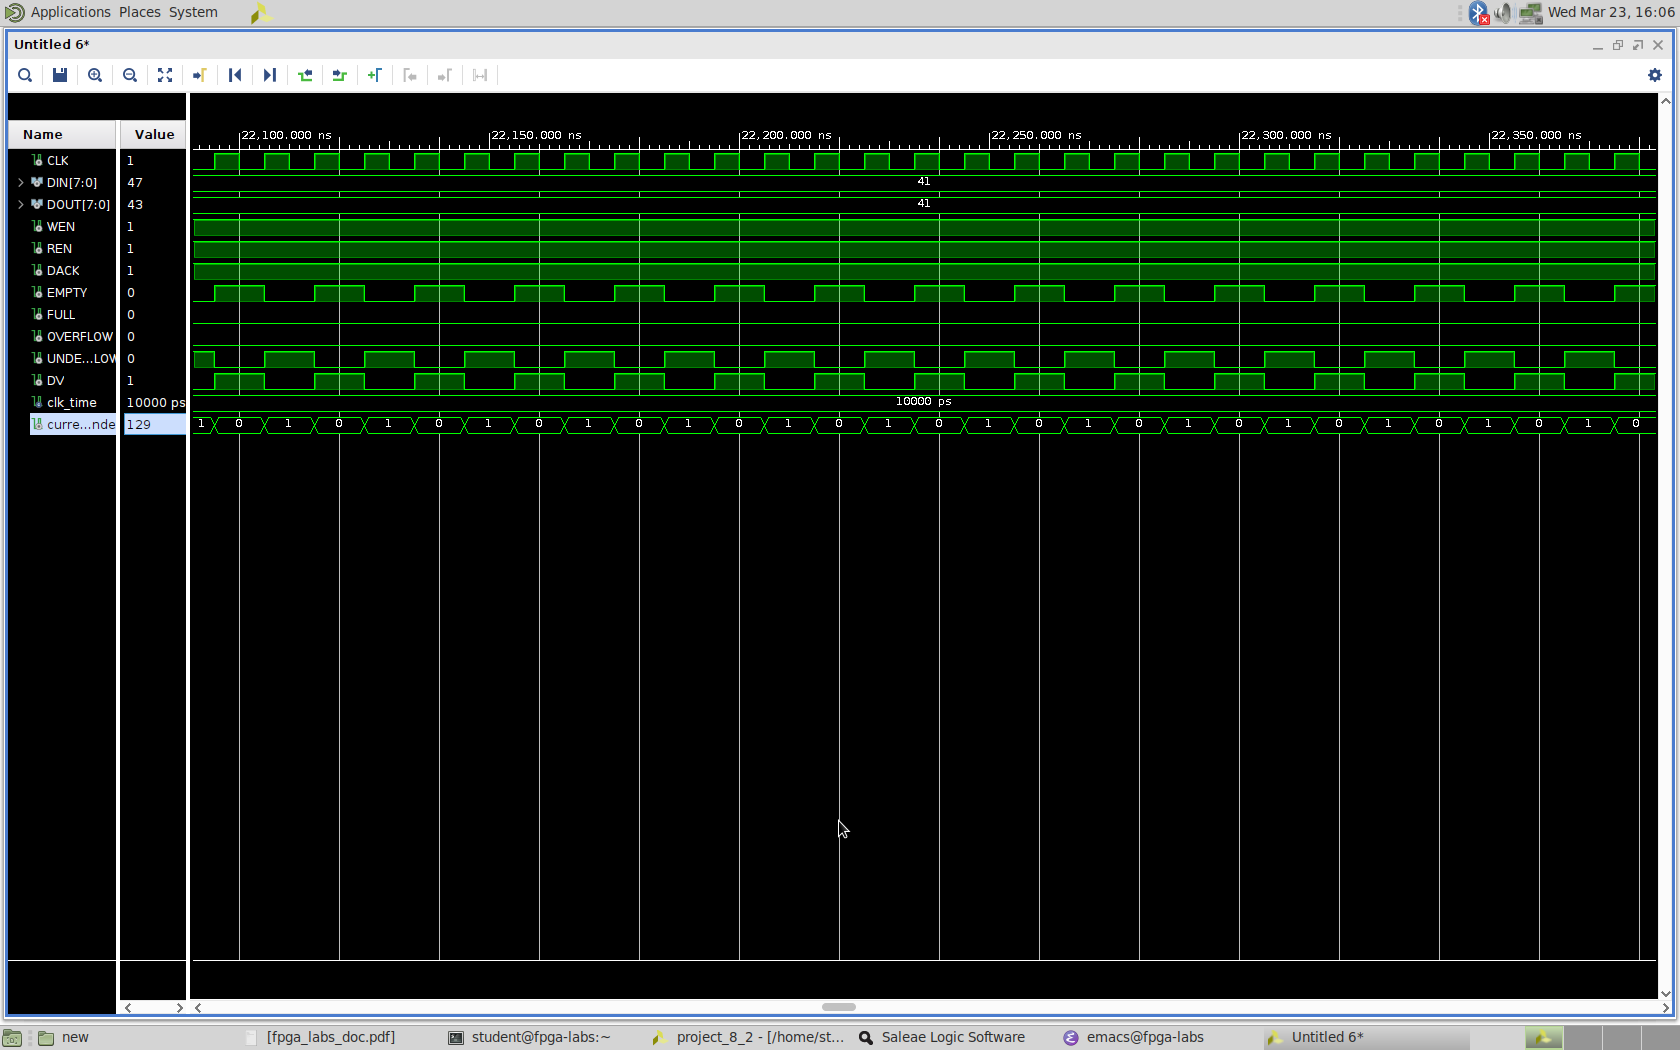
\includegraphics[width=\textwidth]{L8/E2/sim_read_write_underflow_empty.png}
    \caption{Writing and reading from an empty stack. The current address number oscillates between 0 and 1.}
    \label{pic: w and r from e stack}
\end{figure}

\begin{figure}
    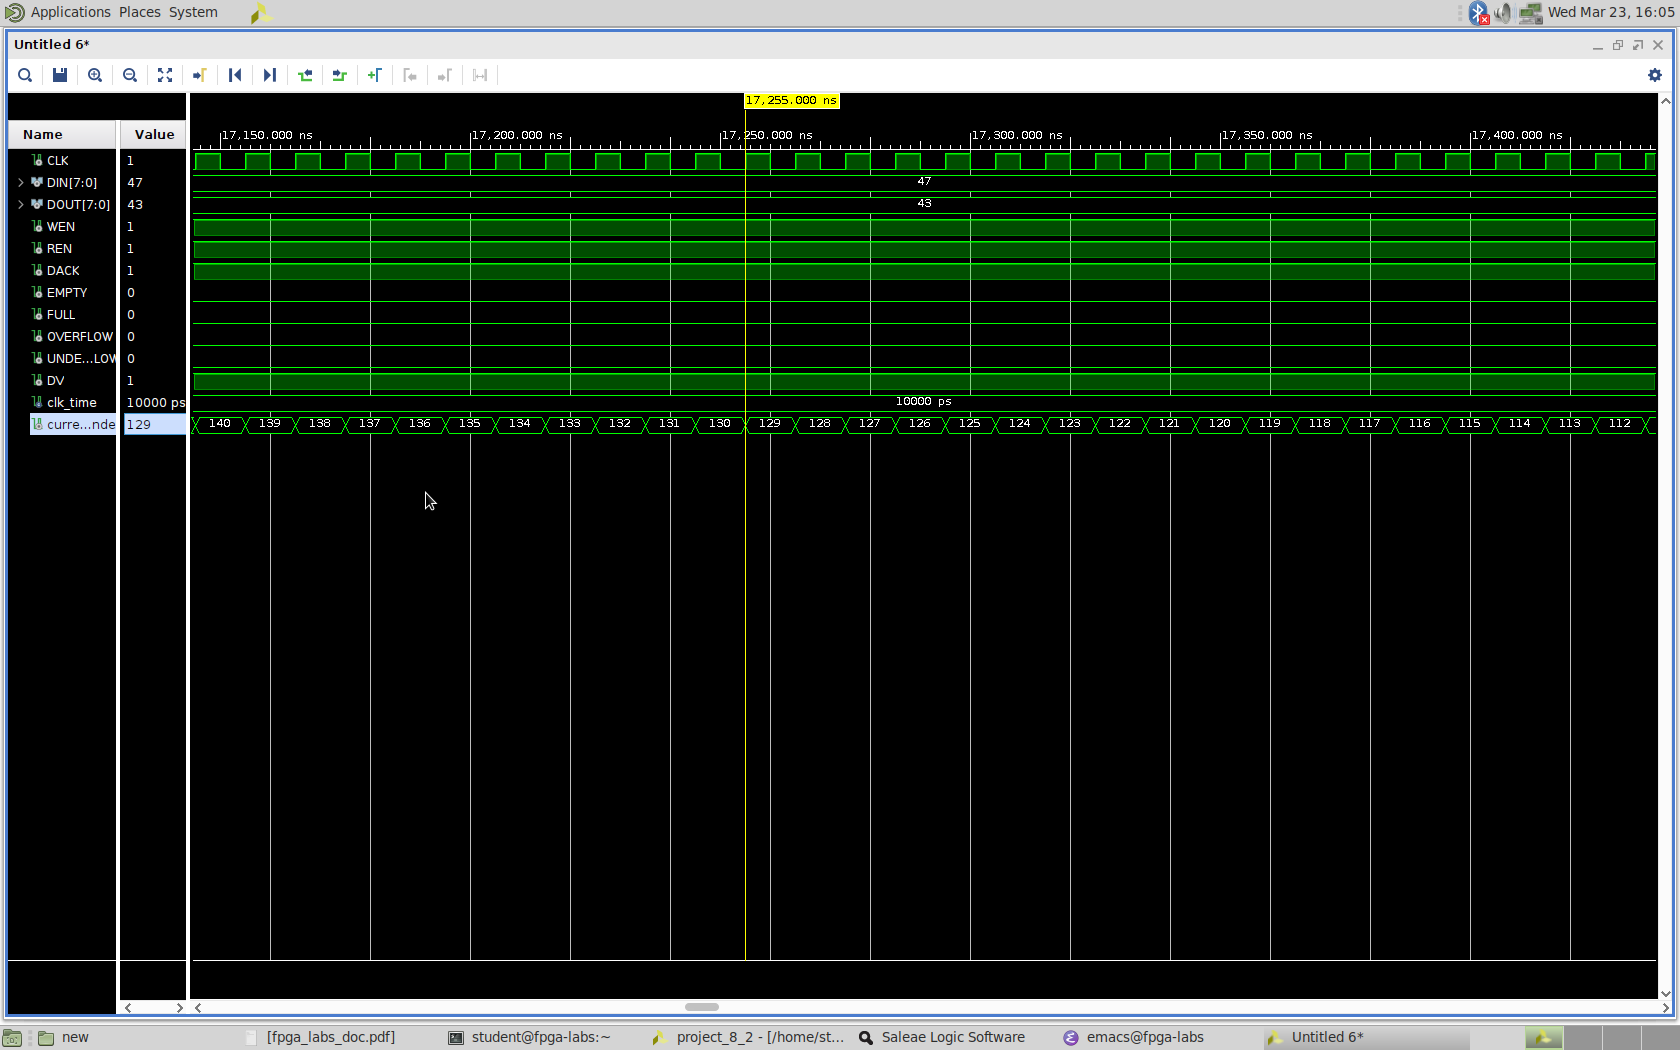
\includegraphics[width=\textwidth]{L8/E2/sim_read_write_full.png}
    \caption{Writing and reading from a full stack. The current address number goes down.}
    \label{pic: w and r from f stack}
\end{figure}

\section{FIFO/queue}

\lstinputlisting[language=VHDL]{L8/E3/src/project_8_3.vhd}